\chapter*{Capítulo 2}
\addcontentsline{toc}{chapter}{\textcolor{ocre}{Capítulo 2}}


\begin{itemize}

 \item 1.	Se invierten 350.000 COP en un depósito a término fijo de 3 años al 28\% nominal anual trimestre vencido. Determinar el monto de la entrega al vencimiento del documento.  \\
       \medskip

 \item 2. Hallar el monto de 480.000 COP en 127 días suponiendo una tasa del 30\% "nominal anual año vencido", use un año de 360 días.\\
       \medskip

 \item 3.¿Qué capital debo invertir hoy para poder retirar un millón de pesos dentro de 18 meses suponiendo que el capital invertido gana el 28\%  nominal anual semestre vencido ?\\

       \textbf{Respuestas:}  674.971,52 COP
       \medskip

 \item 4. ¿Cuál es el valor presente de 800.000 COP en 36 días al 32\% "nominal anual año vencido"? Use un año de 360 días.\\
       \textbf{Respuestas:}  778.094,92 COP
       \medskip

 \item 5. Halle la rentabilidad anual de un documento que se adquiere en 300.000 COP y se vende 6 meses más tarde en 500.000 COP. \\
       \medskip

 \item 6. ¿A qué tasa nominal anual mes vencido se duplica un capital en 2,5 años?  \\
       \textbf{Respuestas:} 2,34\% nominal anual mes vencido
       \medskip

 \item 7. ¿A qué tasa nominal trimestral se triplica un capital en 4 años?\\
       \textbf{Respuestas:} 28,43\% nominal anual trimestre vencido
       \medskip

 \item 8. Una compañía dedicada a la intermediación financiera desea hacer propaganda para captar dineros del público, la sección de mercadeo le dice al gerente de la compañía que una buena estrategia de mercado es duplicar el dinero que depositen los ahorradores. Si la junta directiva de la compañía autoriza pagar por la captación de dinero un máximo de 2,5\% nominal anual mes vencido. ¿Cuánto tiempo debe durar la inversión?  \\
       \textbf{Respuestas:} 28,07 meses
       \medskip

 \item 9. ¿En cuánto tiempo se triplica un capital al 8\% periódico trimestral, sabiendo que el interés solo se paga por trimestres completos?\\
       \textbf{Respuestas:} 15 meses
       \medskip

 \item 10. Decidir la mejor alternativa entre invertir en una compañía de financiamiento comercial que en depósitos a término fijo paga el 28\% nominal trimestral vencido, o invertir en una empresa de turismo que garantiza triplicar el capital en 3 años y 6 meses.\\
       \textbf{Respuestas:} Es mejor la empresa de turismo
       \medskip

 \item 11. Una máquina que actualmente está en uso llegará al final de su vida útil  al final de 3 años, para esa época será necesario adquirir una nueva máquina y se estima costará unos 2'000.000 COP, la máquina que actual opera para esa época podrá ser vendida en 500.000 COP. Determinar el  valor que se debe depositar hoy en un depósito a término fijo de 3 años que garantiza el 7,5\% nominal anual año vencido  \\
       \medskip

 \item 12. a) Hallar una tasa nominal anual trimestre vencido equivalente al 7\% nominal anual trimestre vencido anticipado.\\
       \textbf{Respuestas:} a) 7,527\% nominal anual trimestre vencido \\

       b) Hallar una tasa nominal mensual anticipada equivalente al 3\% efectivo mensual. \\
       \textbf{Respuestas:} b) 2,913\% período mes anticipado
       \medskip

 \item 13. a. Hallar una tasa nominal anual semestre vencido equivalente al 24\% nominal anual trimestral vencido.\\
       \textbf{Respuestas:} a) 24,72\% nominal anual semestre vencido\\

       b. Hallar una tasa nominal anual trimestre anticipado equivalente al 2,5\% periódo mes vencido.\\
       \textbf{Respuestas:} b) 28,56\% nominal anual trimestre anticipado
       \medskip

 \item 14.  a. Hallar una tasa período mes anticipada equivalente al 41,12\% nominal anual año vencido.\\
       \textbf{Respuestas:} a) 2,83\% período mes anticipado  \\

       b. Hallar una tasa nominal anual mes vencido equivalente al 36\% nominal anual mes anticipado.\\
       \textbf{Respuestas:} b) 3,093\% nominal anual mes vencido
       \medskip

 \item 15. a) Dado el 28\% nominal anual trimestre anticipado hallar una tasa nominal semestral equivalente.\\
       \textbf{Respuestas:} a) 31,24\% nominal anual semestre vencido \\

       b. Dado el 27\% nominal anual semestre vencido hallar una tasa nominal anual mes anticipado equivalente.\\
       \textbf{Respuestas:} a) 25,061\% nominal anual mes anticipado
       \medskip

 \item 16. a) Hallar una tasa período año vencido, equivalente al 25\% nominal anual año vencido anticipado.\\
       \textbf{Respuestas:} a) i = 33,33\% periodo año vencido\\

       b) Hallar una tasa efectiva anual anticipada, equivalente al 36\% anual efectivo. \\
       \textbf{Respuestas:} b) $j_{a}$ = 26,47\% nominal anual año vencido\\

       c) Hallar una tasa efectiva anual anticipada, equivalente al 2,5\% periódo mes vencido.\\
       \textbf{Respuestas:} c) $j_{a}$ = 25,64\% nominal anual año vencido
       \medskip

 \item 17. Dado el 15\% periódo semestre vencido hallar una tasa equivalente para un quinquenio.\\
       \textbf{Respuestas:} 304,56\% (período 5 años) na5av
       \medskip

 \item 18. Dado el 208\% período 3 años hallar una tasa periódica equivalente para 2 años.\\
       \textbf{Respuestas:} 111.69\% (período 2 años)  p2av
       \medskip

 \item 19. Dado el 31\% nominal anual 205 días vencido (205 días vencido) hallar una tasa efectiva equivalente anual. Base 365 días.\\
       \textbf{Respuestas:} 33.08079\% nominal anual año vencido
       \medskip

 \item 20. Dado el 40\% nominal anual 185 días vencido (185 días vencido) hallar una tasa efectiva equivalente anual. Base 365 días.\\
       \textbf{Respuestas:} 43.9383467\% nominal anual año vencido
       \medskip

 \item 21. Dado el 35\% nominal anual 160 días vencidio (160 días vencido) hallar una tasa nominal anual 300 días vencido (300 días vencido) equivalente. Base 365 días.\\
       \textbf{Respuestas:} 37.3349\% nominal anual 300 días vencido (300 días vencido)
       \medskip

 \item 22. Dado el 43\% nominal anual 200 días vencido (200 días vencido) hallar una tasa nominal anual 111 días vencido (111 días vencido) equivalente.\\

       a) Base 360 días\\
       b) Base 365 días\\

       \textbf{Respuestas:} a)53,05304\% nominal anual 111 días vencido (111 días vencido), b)52,8799\% nominal anual 111 días vencido (111 días vencido)
       \medskip

 \item 23. Dado el 32\% nominal anual año vencido hallar la tasa nominal 158 días vencidos. \\
       \textbf{Respuestas:} a) 29,500356\% nominal anual 158 días vencido (158 días vencido)
       \medskip

 \item 24. Una persona tiene dos deudas una de 250.000 COP pagadera en 3 meses y otra de 400.000 COP pagadero en 7 meses. Si desea cambiar la forma de cancelarlas mediante dos pagos iguales de X COP c/u con vencimiento en 5 meses y 12 meses respectivamente, determinar el valor de los pagos suponiendo una tasa del 36\% nominal anual mes vencido.\\
       \medskip

 \item 25. Una empresa tiene dos deudas con un banco, la primera deuda es de 100.000 COP con interés del 30\% nominal anual mes vencido, se adquirió hace 6 meses y hoy se vence; la segunda por 200.000 COP al 32\% nominal anual mes vencido se contrató hace 2 meses y vence en 4 meses, debido a la incapacidad de cancelar la deuda, la empresa propone al banco refinanciar su deuda, llegándose a un acuerdo entre las partes de la siguiente forma: Hacer 3 pagos iguales con vencimiento en 6 meses, 9 meses y 12 meses, con una tasa del 33\% nominal anual mes vencido. ¿cuál es el valor de cada pago?\\
       \textbf{Respuestas:} 138.452,64 COP
       \medskip

 \item 26. Un almacén va a ser vendido el 20 agosto. Los inventarios realizados el mismo 20 de agosto arrojaron el siguiente resultado:\\

       a)	En caja 80.000 COP\\
       b)	En bancos 250.000 COP\\
       c)	Cuentas por cobrar \\
       C1 cheque por 65.000 COP para el 30 de septiembre\\
       C2 depósito a término fijo de 6 meses por 235.000 COP e intereses al 28\% nominal anual mes vencido, la inversión se efectuó hace 3 meses.\\
       d)	Mercancías por 950.000 COP\\
       e)	Cuentas por pagar:\\
       D1 cheque por 150.000 COP para el 21 de septiembre\\
       D2 letra por 400.000 COP para el 18 de noviembre.\\

       Con un interés del 30\% nominal anual año vencido usando interés bancario determine el valor del almacén el día de la venta.\\
       \textbf{Respuestas:} 1'074.317 COP
       \medskip

 \item 27. Hoy se contrae una deuda por 500.000 COP con intereses al 30\% nominal anual trimestre vencido y vencimiento en 6 meses y hay una deuda por 800.000 COP contraida hace 3 meses con interés al 32\% nominal anual semestre vencido y vencimiento en 1 año. ¿En qué fecha deberá hacer un pago de 1'700.000 COP para cancelar las deudas suponiendo que el rendimiento normal del dinero es del 2,5\% período mes vencido?\\
       \textbf{ Respuestas:} 9,027 meses
       \medskip

 \item 28. Hallar el tiempo en que debe hacerse un pago de 300.000 COP, para cancelar dos deudas: una de 150.000 COP, con vencimiento en 6 meses y  otra de 150.000 COP con vencimiento en 26 meses. Suponga una tasa del 30\% nominal anual mes vencido.\\
       \textbf{Respuestas:} 1 año, 2 meses y 23 días
       \medskip

 \item 29. Resuelva el problema anterior suponiendo una tasa del 30\% nominal anual trimestre vencido.\\
       \textbf{Respuestas:} 1 año, 2 meses y 24 días
       \medskip

 \item 30. Se deben pagar: 800.000 COP en 3 meses, 1'000.000 COP en 10 meses y 900.000 COP en 15 meses y se van a cancelar en dos pagos el primero por 1'700.000 COP en 9 meses,  ¿en qué fecha deberá pagar 850.510,96 COP para saldar las deudas suponiendo que el dinero rinde el 8\% período vencido?
       \medskip

 \item 31. En el desarrollo de un proyecto hubo necesidad de una inversión inicial de 700.000 COP y se obtuvieron ingresos por 500.000 COP en 3 meses y 450.000 COP a los 10 meses. Hallar la rentabilidad nominal anual mes vencido que generó el proyecto?\\
       \medskip

 \item 32. Una empresa debe cancelar hoy 15 de febrero de 1998 una deuda por 700.000 COP con intereses del 30\% período trimestre vencido adquirida el 15 de agosto de 1997 y otra deuda por 1'000.000 COP obtenida el 15 de diciembre 1997 con vencimiento el 15 de junio 1998 a la misma tasa de la deuda anterior, ante la dificultad de la empresa para cancelar la deuda, el acreedor propone cancelar las deudas con un pago de 200.000 COP ahora y otro de 2'200.000 COP en 10 meses. ¿Cuál es la tasa de interés efectiva anual de refinanciación que se está cobrando?\\
       \medskip

 \item 33. Una empresa tiene tres deudas así:
       \begin{center}
        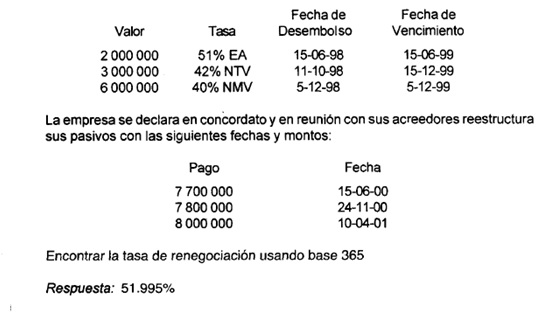
\includegraphics[height=9.2cm]{E2_33}
       \end{center}

\end{itemize}